\documentclass[12pt, a4paper]{article}

% Packages
\usepackage[utf8]{inputenc}
\usepackage[ngerman]{babel}
\usepackage{graphicx}
\usepackage{xcolor}
\usepackage{listings}
\usepackage{float}
\usepackage{svg}
\usepackage{fancyhdr}
\usepackage{tabularx}
\usepackage{geometry}
\usepackage{array}
\usepackage{booktabs}
\usepackage[parfill]{parskip}
\usepackage[hidelinks]{hyperref} % Hyperlinks without color boxes
\usepackage{wrapfig}
\usepackage{placeins}

\geometry{top=2cm, bottom=3cm, left=2.5cm, right=2.5cm}

\author{Robin Ganahl}

\pagestyle{empty}  % No footer or header on the first page

\title{
  \vspace*{-2.5cm} % shift whole header up
  \begin{center}
    \textbf{\LARGE DIPLOMARBEIT} \\ [0.5em]
    \Large Fotobox
  \end{center}
}

\date{} % Remove date

\parindent0pt

% Code style
\definecolor{codegreen}{rgb}{0,0.6,0}
\definecolor{codegray}{rgb}{0.5,0.5,0.5}
\definecolor{codeorange}{rgb}{1.0,0.5,0}

\lstdefinestyle{csharp}{
    language=[Sharp]C,
    backgroundcolor=\color{gray!10},
    commentstyle=\color{codegreen},
    keywordstyle=\color{blue},
    numberstyle=\tiny\color{codegray},
    stringstyle=\color{codeorange},
    basicstyle=\ttfamily\small,
    breakatwhitespace=false,
    breaklines=true,
    captionpos=b,
    keepspaces=true,
    showspaces=false,
    showstringspaces=false,
    showtabs=false,
    tabsize=2,
    frame=single,
    framerule=0.5pt,
    morekeywords={partial, var, value, get, set, async, await}
}
\lstset{style=csharp}


\graphicspath{{images/}}


% Custom footer for the rest of the document
\fancypagestyle{plain}{  % The "plain" style is used for all pages after title
  \fancyhf{}  % Clear header and footer
  \renewcommand{\footrulewidth}{0.4mm}  % Adds a line above the footer
  \fancyfoot[R]{\thepage}  % Page number in the center of the footer
  \fancyfoot[L]{\small DA \textbar\ 2024/25 \textbar\ Fotobox \textbar\ Robin Ganahl}  % Custom text on the left
  \renewcommand{\headrulewidth}{0pt}  % No header line
}

\begin{document}


\maketitle

\vspace{-1cm}

% TODO: ersetzen durch die fertig zusamengabeuta fotobox
\begin{figure}[H]
  \centering
  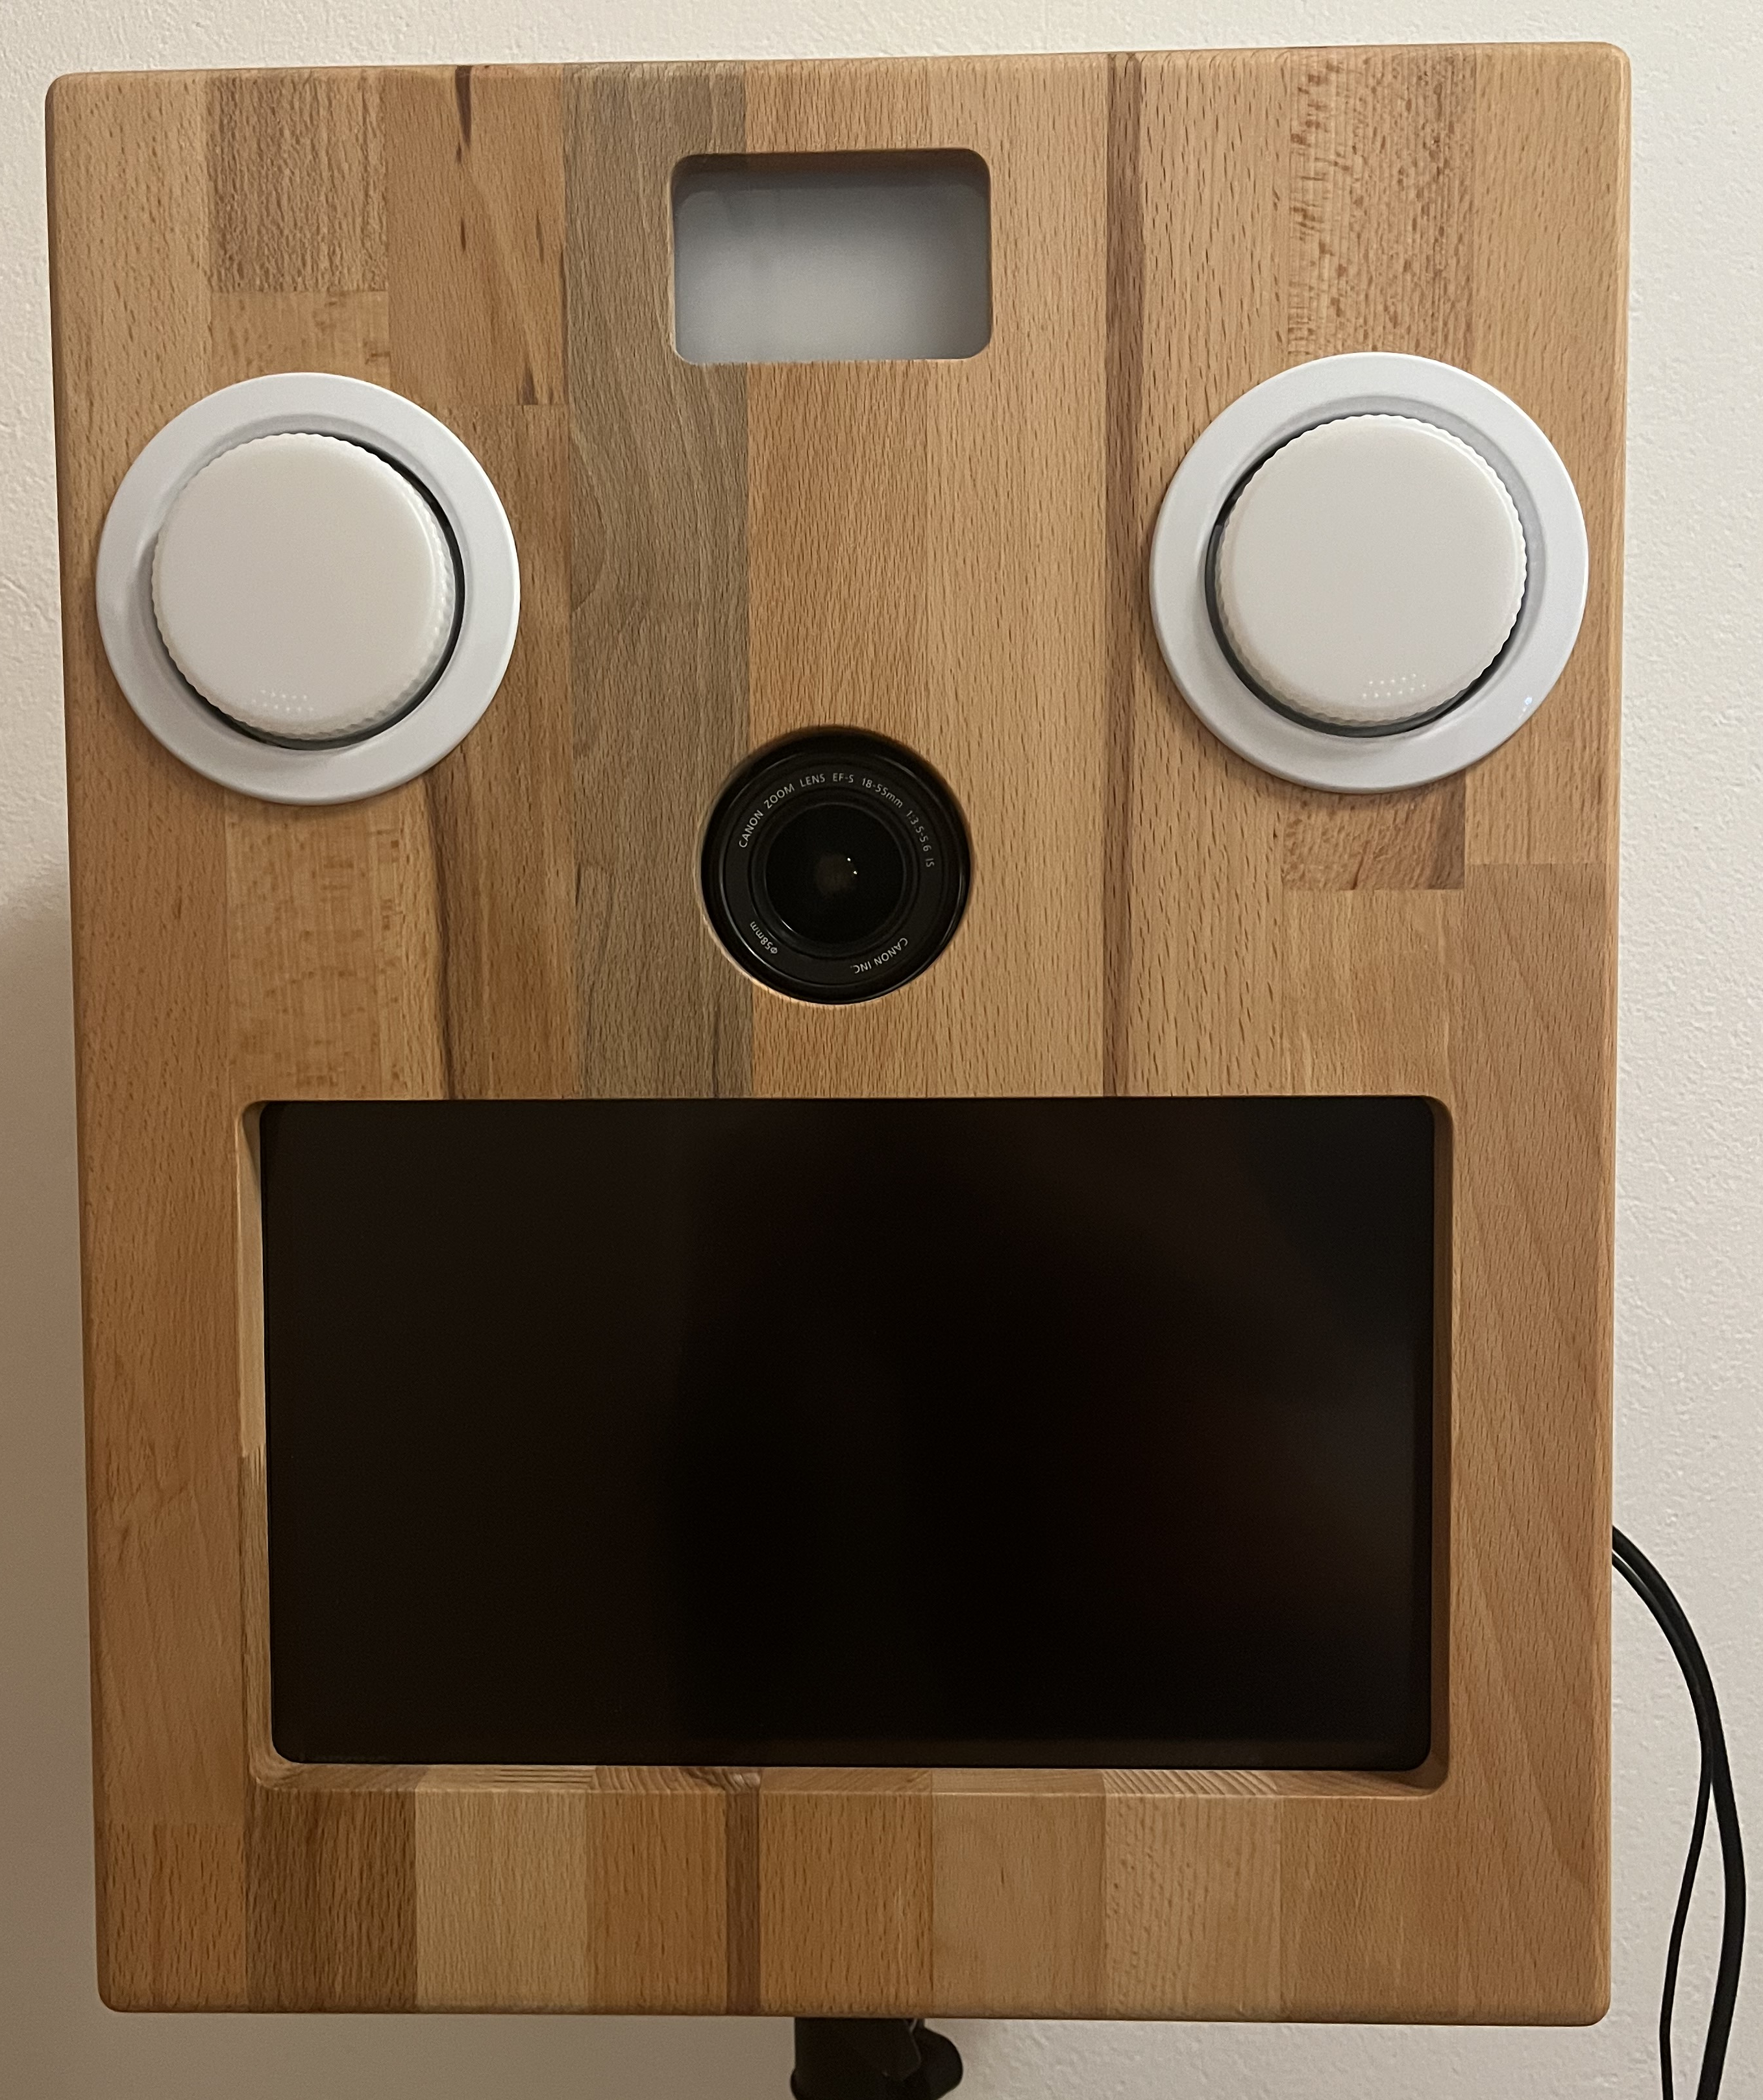
\includegraphics[width=0.7\textwidth]{images/mechanics/fotobox_vorne.JPG}
\end{figure}

\thispagestyle{empty}  % No footer on the first page needs to come after \maketitle

\begin{table}[h!]
    \centering
    \begin{tabular}{l l l}
        \textbf{Ausgeführt im Schuljahr 2024|2025 von:} & & \textbf{Betreuer/in:} \\ 
        \\
        Robin Ganahl & 6/7ABELI & Diem Lukas, DI, BEd. \\ 
    \end{tabular}
\end{table}

\vspace{0.5cm} % Adds space between table and date
Rankweil, am \today
\\
\rule{\linewidth}{0.4mm}  % Creates a line that spans the entire width of the page

\begin{table}[h!]
    \centering
    \begin{tabular}{l @{\hspace{6cm}} l}  % Add horizontal space between the columns
        \textbf{Abgabevermerk:} & \\ 
        \\
        AA original, am 8. April 2025 & Diem Lukas, DI, BEd. \\ 
        \\
        AA digital, am 8. April 2025 & Plattform \\ 
    \end{tabular}
\end{table}

\newpage
\tableofcontents
\newpage

\pagestyle{plain}  % Use custom footer starting from this point

\graphicspath{{images/general}}

\section{Diplomarbeit Dokumentation}

\newpage

\section{Eidesstattliche Erklärung}

Ich erkläre an Eides statt, dass ich die vorliegende Diplomarbeit selbständig
und ohne fremde Hilfe verfasst, andere als die angegebenen Quellen und
Hilfsmittel nicht benutzt und die den benutzten Quellen wörtlich und
inhaltlich entnommenen Stellen als solche erkenntlich gemacht habe.

\vspace{1cm}

Rankweil, am 17.05.2025

\begin{figure}[h!]
    \raggedleft
    \includegraphics[width=0.3\textwidth]{unterschrift.pdf}
\end{figure}

\newpage

\section{Zusammenfassung}

\subsection{Aufgabenstellung}

Viele Fotobox-Programme sind entweder kostenpflichtig und oft sehr teuer, oder 
als Open-Source-Software verfügbar, aber technisch veraltet und schwer anpassbar.
Diese Einschränkungen machen es schwierig, eine kostengünstige und moderne
Lösung zu finden, die den aktuellen Anforderungen entspricht.
Daher habe ich mich entschieden, im Rahmen meines Maturaprojekts ein eigenes
Fotobox-Programm in C\# zu entwickeln und eine passende Fotobox-Hardware zu bauen.
Mein Ziel ist es, eine benutzerfreundliche, flexible und zeitgemäße Alternative
zu bestehenden Lösungen zu schaffen.

\subsection{Umsetzung}

Für die Umsetzung des Projekts habe ich eine moderne Fotobox-Software in C\# entwickelt,
welche auf einem Windows-PC verwendet werden kann. Die Software unterstützt sowohl Webcams,
beispielsweise die im Laptop integrierte Kamera, als auch professionelle Canon-Spiegelreflexkameras.
Die Fotobox-Hardware besteht aus einer hochwertigen Kamera und einem Laptop mit Touchscreen,
der sowohl zur Bedienung als auch zur Verarbeitung der Bilder dient. 
Für die Benutzerinteraktion wurde eine intuitive Oberfläche mit großen,
leicht verständlichen Buttons entwickelt, um die Bedienung so einfach wie
möglich zu gestalten. Die erstellten Bilder können anschließend direkt
ausgedruckt oder über eine Cloud-Anbindung auf einen Server hochgeladen werden.
Von dort aus können sie bequem auf ein Smartphone heruntergeladen werden.

\subsection{Ergebnisse}

Das Projekt führte zu einer voll funktionsfähigen Fotobox, die eine
benutzerfreundliche und moderne Lösung für Veranstaltungen bietet.
Die Software ermöglicht die Steuerung einer Kamera, das Aufnehmen,
Speichern und Teilen von Fotos sowie den direkten Druck. Dank einer intuitiven
Oberfläche ist die Bedienung einfach und effizient.
Ein besonderer Fokus lag auf der Modularität: Das System kann problemlos
um neue Funktionen, wie Filter oder zusätzliche Hardware erweitert werden.
Zudem wurde eine Cloud-Anbindung integriert, sodass Nutzer ihre Fotos direkt
auf ihr Smartphone herunterladen können. Insgesamt entstand eine kostengünstige,
flexible und zeitgemäße Alternative zu bestehenden Fotobox-Lösungen.

\graphicspath{{images/program}}

\section{Programm}

% In diesem Kapitel wird das Programm beschrieben, welches die Fotobox steuert.
% Zuerst grober aufbau mitteld diagramm und beschreibung einzelner komponenten.
% Dann in späteren kapiteln genauere beschreibung.

Das gesamte Fotoboxsystem besteht aus mehreren Komponenten, die möglichst nahtlos
miteinander Arbeiten, um dem Benutzer eine einfache und intuitive Bedienung
zu ermöglichen. 

Im Zentrum steht das Windows-Programm, das die Steuerung der Kamera und des
Druckers übernimmt. Es zeigt das Livebild der Kamera auf dem Laptop an,
verarbeitet die aufgenommenen Bilder und sendet sie an den Webserver.

Ein weiterer Bestandteil ist der Webserver. Dieser organisiert die
aufgenommenen Fotos, stellt eine Benutzeroberfläche bereit, über die die Fotobox
konfiguriert werden kann, und ermöglicht den Download der Bilder.

Das Zusammenspiel dieser Komponenten sowie deren genaue Funktionsweise werden
in den folgenden Kapiteln im Detail erläutert.

\newpage

\subsection{Desktop Applikation}

In dem folgenden Kapitel wird die Desktopapplikation 

\begin{figure}[H]
    \centering
    \includegraphics[width=0.75\textwidth]{Ablauf_Foto_Aufnehmen.drawio.pdf}
    \caption{Ablaufdiagramm der Fotoaufnahme.}
    \label{fig:Ablauf_Foto_Aufnehmen}
\end{figure}

In der Abbildung \ref{fig:Ablauf_Foto_Aufnehmen} ist der Ablauf der Fotoaufnahme dargestellt.
Wenn der Benutzer auf den Auslöser drückt, wird ein Foto aufgenommen.
Anschließend wird das Bild auf dem Laptop angezeigt, und der Benutzer hat die Möglichkeit,
auszuwählen, ob das Foto gespeichert, bzw. gedruckt werden soll, oder nicht.

\graphicspath{{images/mechanics}}

\section{Mechanik}
\begin{figure}[H]
    \centering
    \includegraphics[width=1\textwidth]{fotobox_frontplatte_v2.png}
    \caption{Die erste Version der Frontplatte.}
    \label{fig:frontplatte_v1}
\end{figure}

In der Abbildung \ref{fig:frontplatte_v1} ist die erste Version der Frontplatte zu sehen.
In den löchern eins und zwei sollten jeweils ein Blitz und eine LED Lampe platziert werden,
in dem mittleren Loch mit der Nummer drei sollte die Kamera platziert werden.


Jedoch hat sich herausgestellt, dass durch die seitliche Platzierung des Blitzes
das Motiv einen seitlichen Schatten wirft. Was die Qualität der Bilder deutlich verringert,
da das Bild auch nicht einheitlich ausgeleuchtet wird.

\newpage
\begin{figure}[H]
    \centering
    \includegraphics[width=1\textwidth]{blitz_seitlich.JPG}
    \caption{Beispielbild mit seitlichem Blitz.}
    \label{fig:seitlicher_blitzt}
\end{figure}

In der Abbildung \ref{fig:seitlicher_blitzt} ist zu sehen, dass durch die seitliche Platzierung des Blitzes 
auf der linken seite neben dem Motiv ein Schatten entsteht. Dieser Schatten ist unerwünscht und sollte
durch ein zentrales Blitzlicht vermieden werden.

\begin{figure}[H]
    \centering
    \includegraphics[width=1\textwidth]{blitz_vorne.JPG}
    \caption{Beispielbild mit zentralem Blitz.}
    \label{fig:zentraler_blitz}
\end{figure}

In der Abbildung \ref{fig:zentraler_blitz} ist zu sehen, dass durch die zentrale Platzierung des Blitzes,
das Bild deutlich besser ausgeleuchtet ist und keine seitlichen Schatten entstehen. 

\listoffigures

\end{document}
